Назовём \emph{внешним фотоэффектом} явление испускания электронов вещества под
действием излучения. Эмиссия электронов наблюдается почти у всех веществ, однако
фотоэффект свяжем с металлами, в которых существуют свободные электроны,
удерживаемые внутри металла некоторым энергетическим барьером на границе.
Преодолевая этот барьер, электрон совершает работу выхода (порядка нескольких
эВ), затрачивая часть своей $ E_k $.

В 1888 г. Столетов создал установку с фотоэлементом (см. рис.
\ref{fig:photoel}). Фотоэлемент в виде вакуумной двухэлектродной лампы имеет
металлический катод $ K $, который при освещении его через кварцевое окошко
видимым или ультрафиолетовым светом испускает электроны (благодаря фотоэффекту).
Вылетившие электроны, достигая анода $ A $, создают ток, который фиксируется
гальванометром. Специальная схема подключения источника позволяет изменять
полярность напряжения, подаваемого на фотоэлемент.

\begin{figure}[h]
  \centering
  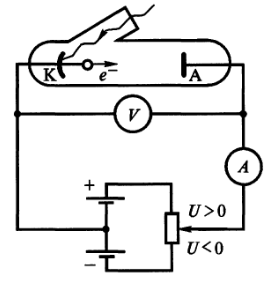
\includegraphics[width=0.8\textwidth]{img/oral-05/photoel.png}
  \label{fig:photoel}
\end{figure}

\begin{figure}[h]
  \centering
  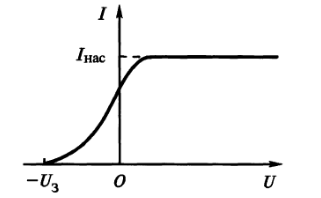
\includegraphics[width=0.8\textwidth]{img/oral-05/vah.png}
  \caption{ВАХ}
  \label{fig:vah}
\end{figure}

При положительном напряжении электрическое поле ускоряет электрон и все
электроны достигают анода, создавая \emph{фототок насыщения} $ I_k $.

Небольшой спад фототока при малых положительных 
напряжениях, который наблюдается в опытах, связан с контактной 
разностью потенциалов между катодом и анодом. Далее при 
обсуждении закономерностей фотоэффекта мы будем пренебрегать
влиянием контактной разности потенциалов.

При $ U < 0 $ не все электроны могут достичь анод, а лишь те, у которых
достаточно кинетической энергии. По графику видно, что она встречается разная.
\emph{Задерживающим напряжением} $ U_{\text{З}} $ назовём такое, при котором
фототок равен нулю.

Измерим $ U_{\text{З}} $ и определим максимальную энергию электрона из
соотношения\footnote{При рассмотрении, например, рентгеновского или $ \gamma $
излучения следует перейти к релятивистской формуле.} 
\[
  E_m = \frac{1}{2}m_0 v_m^2 = eU_{\text{З}}.
\]

Экспериментально были установлены следующие \emph{законы фотоэффекта}:
\begin{enumerate}
  \item Для монохроматического света определенной длины волны
фототок насыщения пропорционален световому потоку, 
падающему на катод.
\item Максимальная кинетическая энергия фотоэлектронов не 
зависит от величины светового потока, а определяется лишь 
частотой излучения.
\item Для каждого вещества катода существует своя граничная
частота $ \nu_K $, такая, что излучение с частотой $ \nu < \nu_K $ фотоэффекта
не вызывает. Эту граничную частоту называют частотой красной
границы фотоэффекта. По шкале длин волн ей соответствует 
длина волны красной границы $ \lambda_K $, такая, что эмиссию электронов из
данного металла вызывает излучение лишь с меньшей длиной
волны ($ \lambda < \lambda_K $).
\end{enumerate}

Классическое рассмотрение проваливается, поскольку, например, должен нарушаться
второй закон, поскольку электроны в этой теории вылетают засчёт силы
электромагнитного поля.

Эйнштейн предложил концепцию фотонов как частиц
излучения, несущих квант энергии. Действительно, в таком
процессе электрон получает всю энергию от фотона, которая 
пропорциональна частоте излучения. Число же вырванных из металла
электронов и, следовательно, фототок насыщения пропорциональны числу падающих на
металл фотонов, которое определяется
величиной потока энергии излучения. Тогда из закона сохранения энергии для
электронов, которым нужно проделать пренебрежимо малую работу для достижения
границы, справедлива формула  
\[
    h\nu = A_B + E_m.
\]
Непосредственно из этого уравнения вытекают второй и третий законы фотоэффекта.
Получаем простые формулы для частоты/длины волны красной границы. Они полностью
определяются $ A_B $.

Возражение о том, что свободный электрон не может поглотить фотон легко
парируется тем фактом, что <<свободные>> электроны в металле взаимодействуют с
атомами решётки.

Назовём \emph{квантовым выходом} $ Y $ число вылетивших электронов на один
падающий фотон. Вблизи красной границы для большинства металлов $ Y = 10^{-4} $
электрон/фотон. Малость квантого выхода обусловлена требованием близости
электронов к границе --- не более $ 0.1 $ мкм. Кроме того, поверхность металлов
сильно отражает излучение. С увеличением энергии фотонов (частоты) $ Y \approx
0.01 \ldots 0.05 $ электрон/фотон. 

С помощью фотоэффекта можно оценить значение $ h $. Для этого запишем уравнение Эйнштейна
в виде 
\[
  eU_{\text{З}} = h\nu - A_B
\]
и увидим, что $ U_{\text{З}} $ линейно зависит от $ \nu $ с угловым
коэффициентом $ h $.

Приборы, в основе устройства которых лежит фотоэффект, 
называют фотоэлементами. Обычный вакуумный фотоэлемент 
выполнен в виде вакуумированной колбы, у которой внутреннюю
поверхность, за исключением небольшого окошечка для доступа
света, покрывает тонкая пленка из металла с малой работой 
выхода (цезий, калий, натрий). Анод представляет собой проволочное
кольцо в центре колбы. Между катодом и анодом прикладывается
ускоряющее напряжение 80\ldots100 В. Фотоэлементы широко 
применяются в технике (фотореле, люксметры, системы звукозаписи
на пленку и др.).
